\section{Evoluce pravidlových systémů}

S rozvojem expertních systémů v 70. a 80. letech přišly i pokusy jak takové systémy znalostí navrhovat jinak než ručně ve spolupráci odborníků na umělou inteligenci s experty v dané problémové doméně. Znalosti v takových systémech, kterým se říká pravidlové, jsou většinou realizovány ve formě pravidel: 

IF (podmínka) THEN (výsledek)

Problém tedy je, jak navrhnout evoluční algoritmus, který bude vyvíjet daná pravidla nebo jejich množiny. Důležitým faktorem, který ovlivňuje návrh takového algoritmu, je typ učení, pro který ho chceme použít. Evoluce pravidlových systémů se historicky uvažuje v kontextu učení s učitelem (např. úlohy klasifikace) a zpětnovazebného učení (vývoj řídících mechanismů pro agenty či roboty). 

Obecně se dá říci, že pro vývoj pravidel v úlohách učení s učitelem máme jedodušší způsob výpočtu a práce s fitness, zatímco v úlohách zpětnovazebného učení (někdy též nazývané on-line učení) je mechanismus interakce pravidlového systému s prostředím a distribuce odměn mezi pravidly složitější.  

Základní principy pro evoluci pravidlových systémů byly položeny v 80.letech 20.století v rámci tzv. Michiganského a Pittsburghského přístupu. Od poloviny 90.let pak mluvíme o nové generaci klasifikačních systémů reprezentované algoritmem Rozčířený klasifikační systém (XCS). 


\section{Michiganský a Pittsburghský přístup}

Prvním, kdo se pokusil skloubit pravidlové systémy a evoluční algoritmy, byl J. Holland, který navrhl koncept \emph{učících se pravidlových systémů}. Pro Hollandův přístup je typické, že uvažoval od počátku problémy zpětnovazebného učení a jeho důraz je tedy na mechanismy distribuce odměny prostředí, zatímco tvar pravidel je co nejjednodušší. Prvním pokusem byl tzv. \emph{Kognitivní systém 1 (CS-1)}, který již obsahuje hlavní rysy toho, čemu dnes říkáme Michiganský přístup, protože ho Holland vyvinul na Michiganské univerzitě. Skupina kolem DeJonga a jeho studentů z Pittsburghské univerzity přišla v algoritmu Učící systém 1 (CS-1) s alternativním přístupem, kterému se dnes říká Pittsburghský, a který je orientován na učení s učitelem a klade větší důraz na tvar pravidel a bohatost evolučních operátorů. 

Hlavním rozdílem mezi oběma přístupy je, že v Hollandově případě je jedincem evoluce jedno pravidlo a jako systém pak slouží celá populace pravidel. V Pittsburgském přístupu se naopak uvažuje s jedincem jako kompletním pravidlovým systémem o několika (desítkách) pravidel. Populace pak obsahuje více takových jedinců, jak jsme z evolučních algoritmů zvyklí.  Výsledkem evoluce je nejlepší jedinec, který představuje kompletní řešení problému. 

\subsection{Michiganský přístup: Hollandův LCS}

Jako typický příklad Michiganského přístupu si ukážeme klasický model Hollandova LCS, což je nástupce algoritmu CS-1,který se snaží řešit adaptivní učení agentů, kde zpětná vazba od prostředí přichází jen pro určité stavy a ne po každé akci agenta. 

Jedincem v Hollandově LCS je jedno pravidlo, které má co nejjednodušší tvar. Podmínka je tvořena bitovou maskou pro detekci jednotlivých vstupů/příznaků a může obsahovat hodnoty 0 - příznak není přítomen, 1 - příznak je přítomen a * - na příznaku nezáleží. Vstupy pravidla jsou buď přímo informace z prostředí poskytované receptory, anebo přiznaky z interních zpráv, které jsou generovány THEN částí pravidel. Tato pravá strana pravidel tedy obsahuje tzv. zprávu, kterou pravidlo, když je aktivováno, vyšle do globální paměti typu black board. Zpráva slouží jednak k zakódování akcí agenta (např. robot postoupí o krok kupředu) a jednak k přenosu informací mezi pravidly (např. robotu dochází baterie). 

Formálně je jeden jedinec reprezentující pravidlo jednoduchým řetězcem v ternární abecedě, takže genetické operátory křížení a mutace jsou standardní a jednoduché. Holland používá také standardní genetický algoritmus, který ale přechod mezi generacemi realizuje jen zřídka --- po mnoha krocích interakce agentů s prostředím --- a nemění celou populaci, ale nahradí jen nějakou část nejhorších jedinců. 

Pro práci s fitness navrhl Holland komplikovaný algoritmus hasičského družstva (bucket brigade), jenž se snaží řešit problém distribuce odměny posloupnosti akcí, které společně vedou k úspěšné interakci agenta s prostředím. Každý jedinec má kromě pravidla ještě číselnou proměnnou, jejíž hodnota určuje sílu pravidla danou jeho úspěšností.   

Již jsme zmínili, že systém obsahuje sdílenou paměť, která uchovává aktuální zprávy jak od prostředí tak od předchozí aplikace pravidel. V jedné iteraci se zprávy z paměti porovnají se všemi pravidly a vyberou se ta pravidla, jejíchž levá strana odpovídá nějaké zprávě. Tato pravidla vsadí část své síly jako poplatek za účast v soutěži, které pravidlo se skutečně uplatní. Hodnota sázky se počítá jako součin síly pravidla, jeho specificity (počtu 0 a 1 na v podmínce) a konstanty. Pravidlo, které vsadí nejvíce, vyhrává a je aplikováno --- v další iteraci umístí svou zprávu do paměti, ale zároveň musí svou sázku zaplatit. Tato hodnota je pak distribuována mezi pravidla, která byla aplikována v minulých krocích. Tím dochází k tomu, že pravidla, která jsou součástí řetězce akcí vedoucího k dobrému výsledku, posilují (metafora řady hasičů předávající si vědro).

\begin{figure}
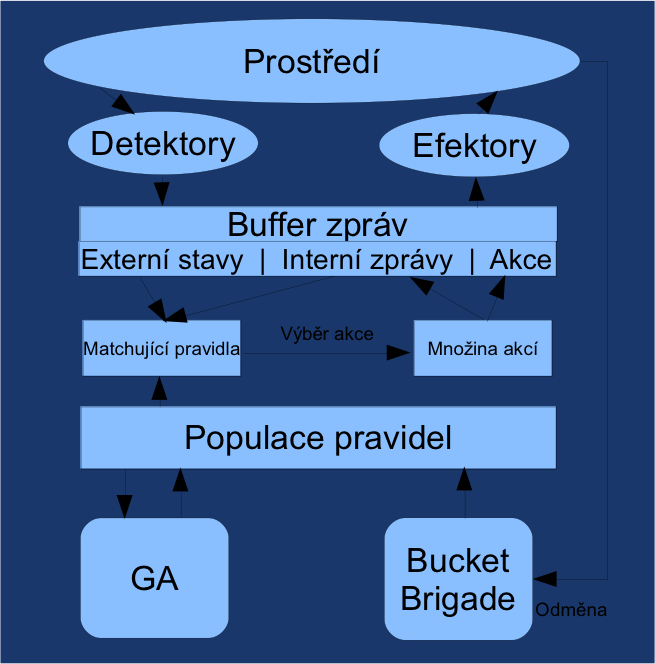
\includegraphics{graphics/bucketbrigade.png}
\caption{Hollandův LCS s algoritmem požárního družstva.}
\end{figure}


\subsection{Pittsburghský přístup: GIL}

Jako příklad Pittsburgského přístupu uvedeme sytém GIL, který je praktickým návrhem evoluce binárního klasifikačního systému, který je celý reprezentován jedincem v evolučním algoritmu. Věnujeme se hlavně reprezentaci jedince a operátorům, kterých je velké množství a pracují na různých úrovních.

Jedinec je tedy v tomto systému množina pravidel, které klasifikují do jedné třídy, pravá strana je vždy stejná a proto ji můžeme v jedinci zanedbat. Každé pravidlo si můžeme představit jako disjunkci komplexů, kde každý komplex je konjunkce seletorů z jedné proměnné. Selektor reprezentuje množinu hodnot proměnné a je reprezentován bitovou mapou. 

((X=A1)AND(Z=C3)) OR((X=A2)AND(Y=B2))

[001|11|0011 OR 010|10|1111]

Uveďme stručně výčet operátorů, které se podílejí na úpravách a rekombinacích jedinců, spíše než o mutacích a kříženích mluvíme o úrovních, na kterých operátory pracují.

\begin{description}

\item{Operátory na úrovní jedince:}
výměna pravidel, kopírování pravidel, generalizace pravidla, smazání pravidla, specializace pravidla, zahrnutí jednoho pozitivního příkladu

\item{Operátory na úrovni komplexů:} 
rozdělení komplexu na 1 selektoru, generalizace selektoru (nahrazení 11...1), specializace generalizovaného selektoru, zahrnutí negativního příkladu

\item{Operace na selektorech:}
Mutace 0<->1, rozšíření 0->1, zúžení 1->0, 

\end{description}


\section{ZCS a XCS}

\subsection{Klasifikační systém nulté úrovně}

V roce 1994 navrhl Wilson výrazně zjednodušenou verzi LCS, kterou nazval učícím se klasifikátorem nulté úrovně (ZCS). Hlavnim rysem algoritmu bylo nahrazení distribuce odměny požárním družstvem pomocí přehledného a jednuššího algoritmu, a zavední nového operátoru pokrytí. 

ZCS v každém kroku identifikuje množinu $M$ (matching) pravidel, která jsou aplikovatelná na daný stav prostředí, z nich se vybere to, které se aplikuje čistě na základě fitness jednotlivých pravidel. Všechna pravidla z $M$, která navrhují stejnou akci jako vítězné pravidlo, tvoří pak množinu $A$ (action set). 

Malý zlomek fitness každého pravidla z $A$ je odečten a připraven k redistribuci. Nasčítané části fitness jsou zmenšeny o konstantu GAMMA. Systém si pamatuje členy množiny $A$ z předchozí iterace, mezi které je tato hodnota rovnoměrně rozdělena. 

Pokud systém v aktuálním kroku obdrží odměnu od prostředí, je od ní odečtena malá konstanta a zbytek je rovnoměrně rozdělen mezi členy aktuální množiny $A$. 

Nakonec je ještě zmenšena fitness pravidel z množiny $M-A$ (těch, která jsou aplikovatelná na danou situaci, ale navrhují jinou akci než vítězné pravidlo) o malý faktor $\tau$. 

Vlastní prohledávání je realizováno kombinací stabilního GA (steady-state GA) a operátoru pokrytí. V každém kroku je s určitou pravděpodobností realzována jedna iterace genetického algoritmu, který ruletovou selekcí vybere dva rodiče, vygeneruje dva potomky, a těmi nahradí dva jedince z populace, vybrané opět ruletovou selekcí. Rodiče předjí potomkům polovinu své fitness.

Operátor pokrytí se aplikuje tehdy, když je množina M v daném kroku prázdná (nebo pokud obsahuje jen podprůměrné jedince), jeho cílem je zajistit, aby celý systém pokrýval co nejvíce případů, které prostředí poskytuje. Operátor pokrytí vygeneruje pravidlo s podmínkou odpovídající aktuálnímu vstupu a náhodnou akcí na pravé straně. 

\subsection{Rozšířený klasifikační systém}

Dodnes nejúspěšnějším přístupem v oblasti klasifikačních systémů je druhý algoritmus navržený Wilsonem, tak zvaný rozšířený klasífikační systém (XCS). Autor v něm explicitně aplikoval principy zpětnovazebného Q-učení, které se snaží o úplnost reprezentace problému výběru akce. Algoritmus byl navržen po zkušenostech se ZCS, který, ač byl na řadě úloh úspěšný, vykazuje tendenci soustředit prohledávání jen do oblastí přinášejících velkou odměnu od prostředí. 
Algoritmus XCS nepočíta fitness pravidel na základě hodnotz této odměny, ale na přesnosti předpovědi pravidel. 

Ke každému pravidlu je přiřazena trojice hodnot --- fitness $F$, chyba $\epsilon$ a predikce $p$. Algoritmus zpětnovazebného učení pak upravuje tyto hodnoty následujícím způsobem:  

V každém kroku se identifikuje množina $M$ a pro každou akci $a$ v $M$ se spočte predikce systému jako průměr predikcí pravidel v každé množině $A$ vážený jejich fitness. Odpověď systému se pak stanoví deterministicky nebo s náhodným faktorem. Pokud je množina $M$ prázdná, použije se operátor pokrytí.  

V následujících pěti krocích se pak upraví fitness a další parametry pravidel podle relativní přesnosti pravidla v dané množině $A$.

\begin{enumerate}
\item aktualizuj chybu každého pravidla: $\epsilon_j = \epsilon_j + \beta \left( \left| P - p_j \right| - \epsilon_j \right)$

\item aktualizuj predikci každého pravidla: $p_j = p_j + \beta (P-p_j)$

\item spočti přesnost pravidla $\kappa_j$ jako: $\kappa = \alpha (\epsilon_0/\epsilon)^v$, anebo $\kappa=1$ pro $\epsilon < \epsilon_0$

\item urči relativní přesnot pravidla $\kappa_j\prime$ jako podíl jeho přesnosti a součtu všech přesností pro danou $A$.

\item Aktualizuj fitness $F_j$ na základě relativní přesnosti pomocí moyennovy adaptivní procedury: 

Pokud už fitness byla aktualizována $1/\beta$ krát,
 $F_j = F_j + \beta(\kappa_j\prime - F_j).$ 
 
Jinak nastav $F_j$ jako průměr aktuální a předchozí hodnoty
$kappa_j\prime$.
\end{enumerate}

Nakonec se maximální hodnota $P(a_i)$ zmenší o faktor $\gamma$ a použije se k aktualizaci pravidel z předchozího kroku.

Genetický algoritmus je opět stabilního typu, ale navíc pracuje s faktorizací prostoru pravidel do množin $A$, jde tedy o nikový GA vybírající pravidla z aktuální množiny $A$. Nahrazovaná pravidla jsou vybírána globálně s ohledem na vyvážení velikostí jednotlivých $A$. Pro danou množinu $A$ se rozhoduje o tom, zda se GA aplikuje na základě průměrného času, kdy se naposledy daná nika A podílela na genetickém algoritmu. 

Systém XCS se od původního návrhu dočkal mnoha rozšíření a vylepšení, jako jsou UCS (sUpervised classifier system) vhodný pro učení s učitelem, a jeho další varianty ExSTraCS v. 1 a 2, které byly úspěšné v řešení těžkých praktických problémů. Systém XCSF je zase rozšířením XCS pro problémy aproximace funkcí. 

